%%%%%%%%%%%%%%%%%%%%%%%%%%%%%%%%%%%%%%%%%
% Presentation Template
% LaTeX Template
% Version 1.0 (2023-02-08)
%
% This template was adapted by:
% Jonathan Decker (jonathan.decker@uni-goettingen.de)
% From a template made by:
% Julian Kunkel (julian.kunkel@gwdg.de)
%
%%%%%%%%%%%%%%%%%%%%%%%%%%%%%%%%%%%%%%%%%
\documentclass[compress,aspectratio=169]{beamer}

% make sure the theme file is on this path
\usepackage{../assets/beamerthemeGoettingen}

\addbibresource{ref.bib}
\graphicspath{{../}{../assets/}}

% --- document configuration ---
\newcommand{\mytitle}{Rust for HPC Applications}
% Leave empty for no subtitle
\newcommand{\mysubtitle}{An Practical Introduction in Rust Performance Engineering}
\newcommand{\myauthor}{Lars Quentin}
\newcommand{\myauthorurl}{lquenti.de}
\newcommand{\myvenue}{Recent Trends in High-Performance Data Analytics}
% For example, use \today
\newcommand{\mydate}{29.06.2023}
% For example, Institute for Computer Science / GWDG
\newcommand{\myinstitute}{GWDG / CIDAS}

\configuretitlepage

\usepackage{listings}



\begin{document}

\begin{frame}[plain]
	\titlepage
\end{frame}

\begin{frame}{Overview}
\tableofcontents
\end{frame}

\section{Introduction}

\begin{frame}{Learning Objectives}
  \begin{itemize}
    \item Why Rust is a good fit for HPC.
    \item How to do the following things in Rust:
      \begin{itemize}
        \item Microbenchmarking
        \item Full Application Benchmarking
        \item Analyze generated Assembly
        \item Compiler Optimizations
        \item Statistical Profiling
        \item CI benchmarking
        \item Parallelism
      \end{itemize}
  \end{itemize}
\end{frame}

% TODO FIX CITATIONS
\begin{frame}{Why Rust is a good fit for HPC}
  \begin{itemize}
      \pause
    \item Its like modern C++ enforced by the compiler
      \begin{itemize}
        \item RAII-based memory management
        \item References are like \texttt{std::unique\_ptr}
      \end{itemize}
      \pause
    \item Great Python / C++ interoperability
      \pause
    \item Allows for very low level control; even supports bare metal deployment.
      \pause
    \item Mature compiler optimizations through LLVM backend
      \pause
    \item Many modern concepts from functional programming
      \begin{itemize}
        \item immutability by default
        \item Traits/typeclasses instead of inheritance
        \item exhaustive pattern matching
        \item Algebraic data types
        \item No Nullability
      \end{itemize}
      \pause
      \item Developers' most loved language for the 7th year according to StackOverflow \cite{sosurvey}
  \end{itemize}
\end{frame}

\begin{frame}{Problem: Quadratic Matrix multiplication}
  \begin{columns}
    \begin{column}{0.5\textwidth}
      Let $A, B \in \mathbb{R}^{n\times n}, n \in \mathbb{N}$. Then $C \in \mathbb{R}^{n \times n}$ is defined as
      \[
        C_{ij} := \sum_{k=1}^n A_{ik} \cdot B_{kj}
      \]
      i.e. $C_{ij}$ is the dot product of the $i$-th row of $A$ and the $j$-th column of $B$.
    \end{column}
    \begin{column}{0.5\textwidth}
      \begin{figure}
        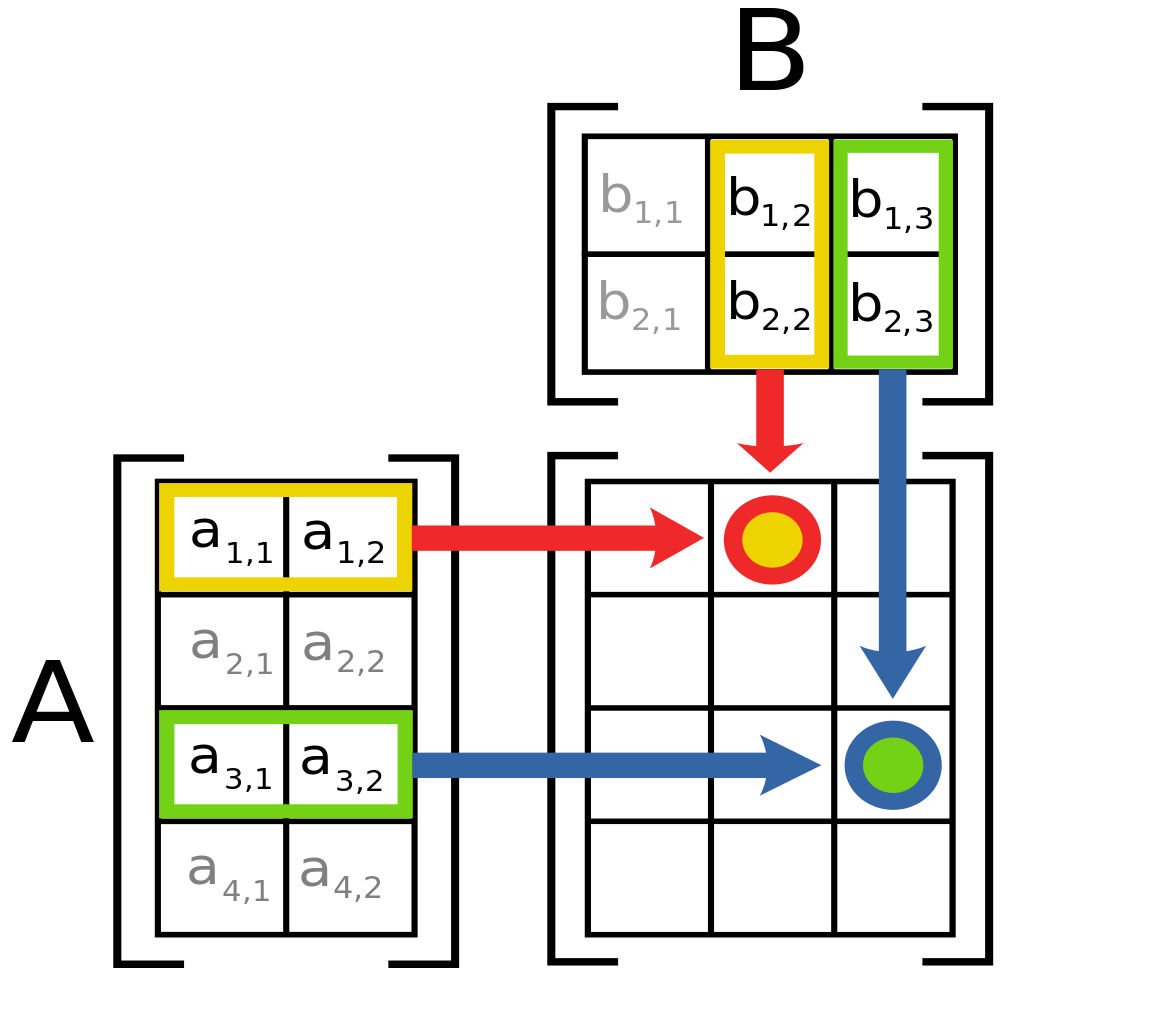
\includegraphics[width=0.8\textwidth]{../assets/Matrix_multiplication_diagram_2.svg.png} \cite{matmulvis}
      \end{figure}
    \end{column}
  \end{columns}
\end{frame}

\section{Simplified Problem}

\begin{frame}[fragile]{Simplified Problem: $3 \times 3$ Matrix}
  \begin{tcolorbox}[title=First Implementation]
    \footnotesize\inputminted[xleftmargin=1em,linenos]{rust}{../assets/first_impl.rs}
  \end{tcolorbox}
\end{frame}
% TODO: MENTION THAT ONE COULD IMPROVE REF VS VAL here.
% This could result in a performance boost
% But how can we make sure about that?

\begin{frame}{Microbenchmarking}
  \begin{block}{Native Benchmarking: \texttt{cargo bench} \cite{cargobench}}
    \begin{itemize}
      \item Not stable (nightly only)
      \item No regression testing or visualizations
      \item No clear roadmap to become stable \cite{cargounstable}
      \item \texttt{cargo-benchcmp} \cite{benchcmp} for comparing benchmarks
    \end{itemize}
  \end{block}
  \pause
  \begin{block}{\texttt{criterion.rs} \cite{criterion}}
    \begin{itemize}
      \item Uses statistical analysis for regression significance
      \item Blocks constant folding
      \item HTML report with plotting through \texttt{gnuplot} \cite{gnuplot}
      \item \texttt{cargo-critcmp} for comparing benchmarks \cite{critcmp}
    \end{itemize}
  \end{block}
\end{frame}

\begin{frame}{Benchmarking Full Applications}
  \begin{columns}
    \begin{column}{0.5\textwidth}
      \begin{block}{Hyperfine \cite{hyperfine}}
        \begin{itemize}
          \item Statistical analysis / outlier detection
          \item Warmup runs
          \item Cache clearing commands available
          \item Export to different formats such as JSON or CSV
          \item Supports parametrized benchmarks
          \item Various Pythonscripts for visualization
        \end{itemize}
      \end{block}
    \end{column}
    \begin{column}{0.5\textwidth}
      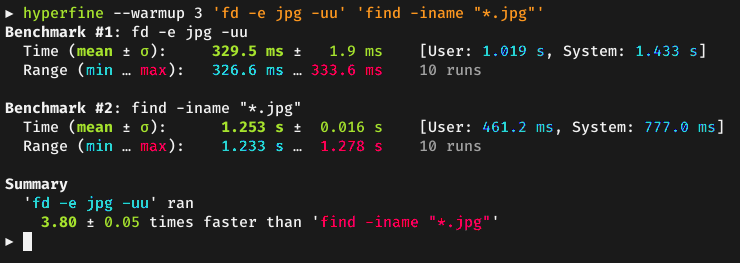
\includegraphics[width=\textwidth]{../assets/hyperfine.png} \cite{hyperfine}
    \end{column}
  \end{columns}
\end{frame}

\begin{frame}{Benchmarking Results (-O3)}
    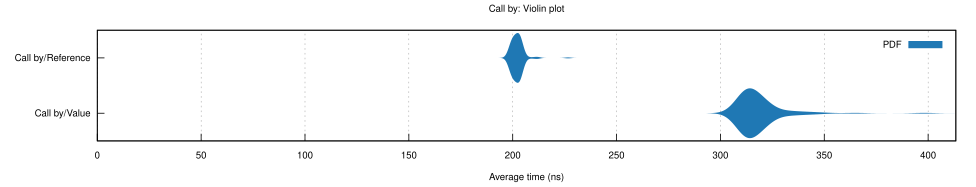
\includegraphics[width=\textwidth]{../assets/first_violin.png}
  \begin{columns}
    \begin{column}{0.7\textwidth}
  \begin{table}[h]
\centering
\begin{tabular}{|l|c|c|c|}
\hline
& \textbf{Mean} & \textbf{Std. Dev} & \textbf{Median} \\
\hline
\textbf{Call By Reference} & 202.31 ns & 3.5063 ns & 201.96 ns \\
\hline
\textbf{Call By Value} & 318.48 ns & 12.173 ns & 314.59 ns \\
\hline
\end{tabular}
\end{table}
    \end{column}
    \begin{column}{0.3\textwidth}
      Total Improvements:\\
      Mean: 57.42\%\\
      Median: 55.77\%
    \end{column}
  \end{columns}
\end{frame}

\begin{frame}[fragile]{Next Improvement: Static Stack Arrays}
  \begin{tcolorbox}[title=Static Stack Arrays]
    \footnotesize\inputminted[xleftmargin=1em,linenos]{rust}{../assets/less_heap_allocation.rs}
  \end{tcolorbox}
  \begin{columns}
    \begin{column}{0.7\textwidth}
  \begin{table}[h]
    \centering
    \begin{tabular}{|l|c|c|c|}
      \hline
      &\textbf{Mean} & \textbf{Std. Dev} & \textbf{Median}\\
      \hline
      \textbf{Call By Value} & 318.48 ns & 12.173 ns & 314.59 ns \\
      \hline
      \textbf{Static Arrays} & 8.0685 ns & 254.42 ps & 8.0121 ns\\
      \hline
      \end{tabular}
  \end{table}
    \end{column}
    \begin{column}{0.3\textwidth}
      Total Improvements:\\
      Mean: 3847.2\%
      Median: 3826.44\%\\
    \end{column}
  \end{columns}
\end{frame}

\begin{frame}{Next Improvement: 1 vs 2 derefs}
  \begin{tcolorbox}[title=Reduce the amount of Dereferences]
    \footnotesize\inputminted[xleftmargin=1em,linenos]{rust}{../assets/less_derefs.rs}
  \end{tcolorbox}
  \begin{columns}
    \begin{column}{0.7\textwidth}
  \begin{table}[h]
    \centering
    \begin{tabular}{|l|c|c|c|}
      \hline
      &\textbf{Mean} & \textbf{Std. Dev} & \textbf{Median}\\
      \hline
      \textbf{Call By Value} & 318.48 ns & 12.173 ns & 314.59 ns \\
      \hline
      \textbf{Less Derefs} & 7.7821 ns & 182.79 ps & 7.7775 ns \\
      \hline
      \end{tabular}
  \end{table}
    \end{column}
    \begin{column}{0.3\textwidth}
      % Note that this is the calculated increase
      Total Improvements:\\
      Mean: 3993.57\%\\
      Median: 3944.87\%
    \end{column}
  \end{columns}
\end{frame}
% TODO Muendlich: Bei dem Spielproblem ist der Code so uebersichtlich dass wir noch den Assembler analysieren koennen

\begin{frame}{Assembly 1: Compiler Explorer \cite{godbolt}}
  \begin{figure}[h]
    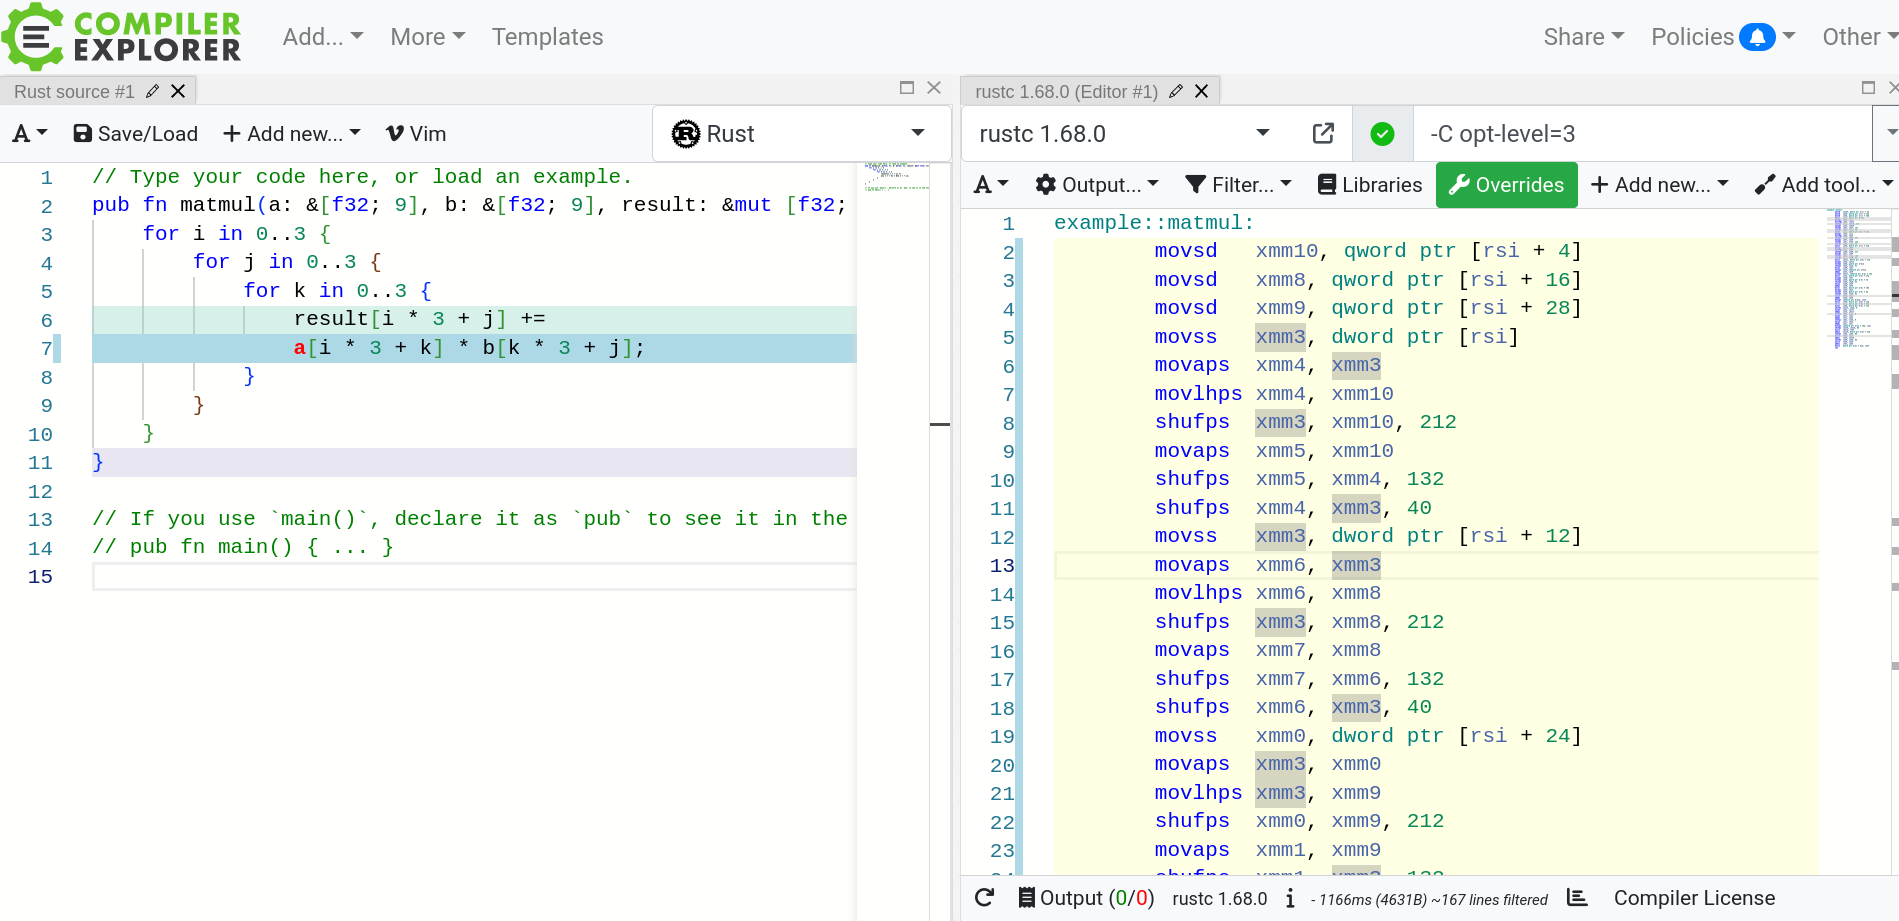
\includegraphics[width=\textwidth]{../assets/compilerexplorer.png}
  \end{figure}
\end{frame}

\begin{frame}{Assembly 2: \texttt{cargo-show-asm} \cite{cargo-asm}}
  \begin{columns}
    \begin{column}{0.5\textwidth}
      \begin{itemize}
        \item Allows to view Assembly or LLVM-IR
        \item Can query single functions
        \item Can also resolve trait implementations
      \end{itemize}
    \end{column}
    \begin{column}{0.5\textwidth}
    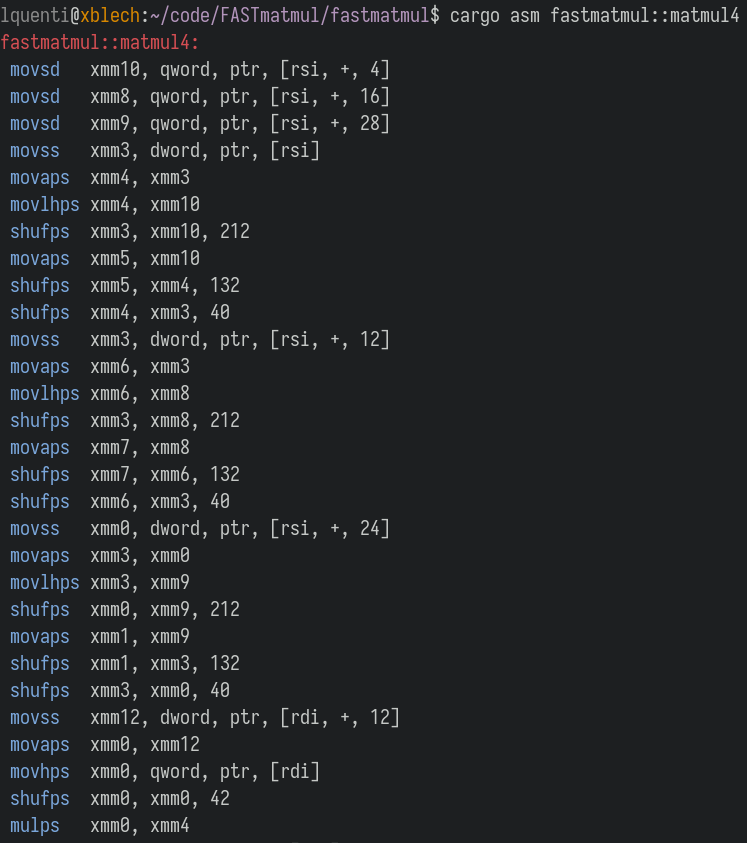
\includegraphics[height=.9\textheight]{../assets/cargoasm.png}
    \end{column}
  \end{columns}
\end{frame}

\begin{frame}{Assembly 3: Loop Unrolling and Function Inlining}
  \begin{block}{Loop Unrolling}
    \begin{itemize}
      \item Was already applied in our case
      \item Tooling: \texttt{unroll} \cite{unroll} provides a macro for creating unrolled rust code.
      \item For dynamic length loops: \texttt{-C llvm-args="-unroll-threshold=N"}
        \begin{itemize}
          \item Do not apply without benchmarking!
        \end{itemize}
    \end{itemize}
  \end{block}
      \pause
  \begin{block}{Function Inlining}
    \begin{itemize}
      \item Was not applied in our case
      \item But compiler hints exist: \texttt{\#[inline(/always/never)]} \cite{perfbook}
    \end{itemize}
  \end{block}
\end{frame}

\section{Real Problem}

\begin{frame}{Introduction Real Problem}
  \begin{itemize}
    \item \textbf{Task:} You get introduced to a scientific problem which is too slow.
      \pause
    \item Why is this so slow?
      \pause
    \item How do I figure this out?
      \pause
    \item \textbf{Solution: Profiling}
  \end{itemize}
\end{frame}

\begin{frame}{Profiling}
  \begin{itemize}
    \item Since Rust produces normal binaries, most profilers just work.
      \begin{itemize}
        \item Including:
          \begin{itemize}
            \item \texttt{perf} \cite{perfwiki}
            \item \texttt{cachegrind} \cite{valgrind}
            \item ...
          \end{itemize}
        \item \texttt{rustfilt} \cite{rustfilt} can demangle all symbols.
      \end{itemize}
      \pause
    \item Here, we will use \texttt{cargo-flamegraph} \cite{cargoflamegraph} and later \texttt{iai} \cite{iai}.
  \end{itemize}
\end{frame}

\begin{frame}{Cargo flamegraph}
  \begin{columns}
    \begin{column}{0.5\textwidth}
    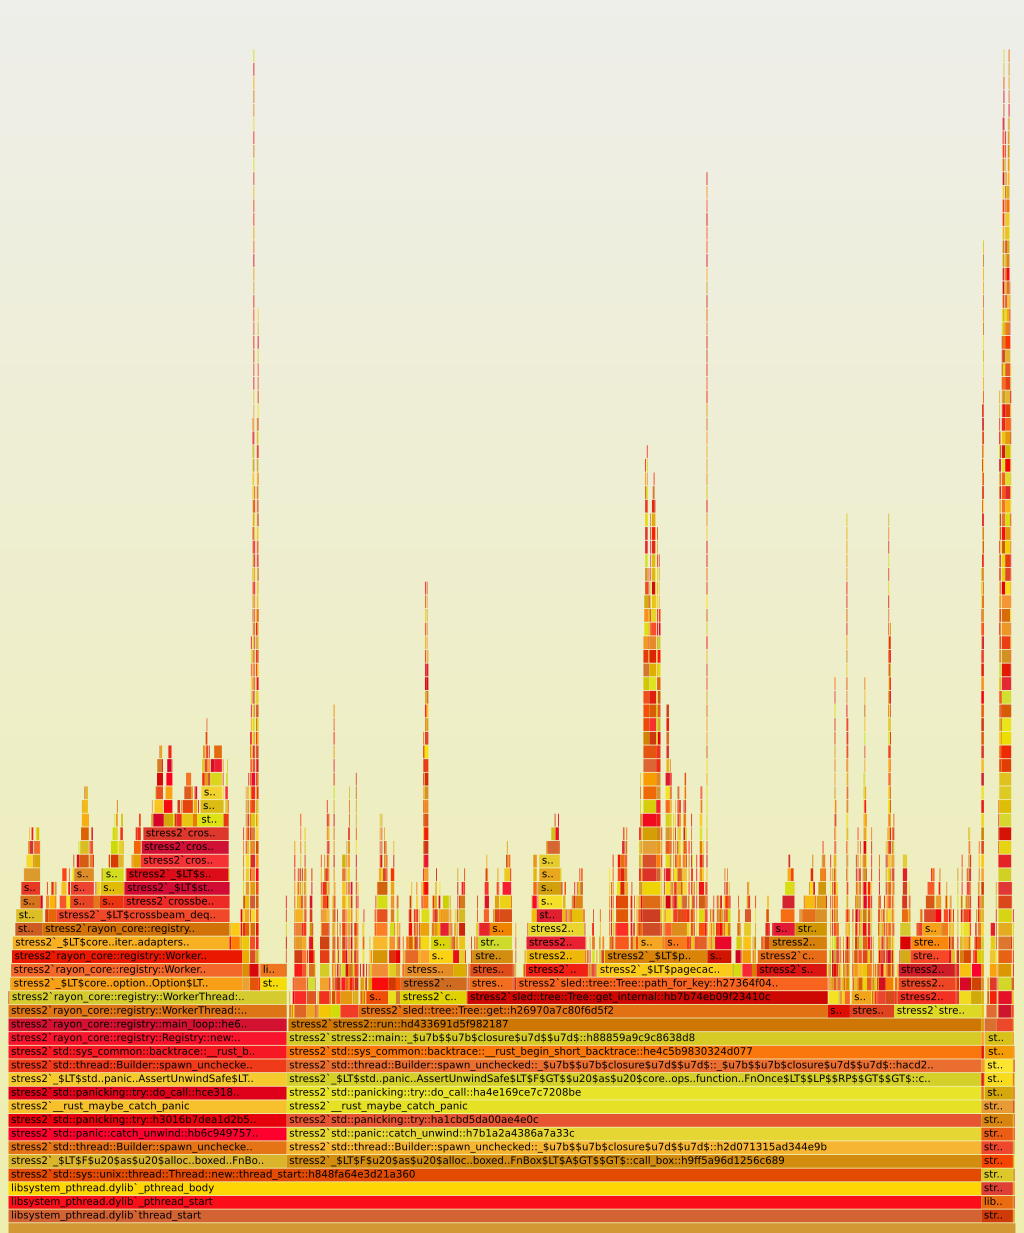
\includegraphics[height=.9\textheight]{../assets/flamegraph.png}
    \end{column}
    \begin{column}{0.5\textwidth}
  \begin{itemize}
    \item Statistical Profiler
      \begin{itemize}
        \item Interrupts randomly
        \item Looks at the stack
        \item Then it can approximate how much time is spent in each function
      \end{itemize}
    \item Uses \texttt{perf} internally
  \end{itemize}
    \textbf{Our Result:} Lets assume the problem was a quadratic $n\times n$ matrix multiplication!\\
    For the benchmarks, we assume $n=1024$.
    \end{column}
  \end{columns}
\end{frame}

\begin{frame}[fragile]{Unoptimized code}
  \begin{tcolorbox}[title=Unoptimized Version]
    \footnotesize\inputminted[xleftmargin=1em,linenos]{rust}{../assets/01nxn.rs}
  \end{tcolorbox}
\end{frame}

\begin{frame}[fragile]{Applying our previous knowledge}
  \begin{tcolorbox}[title=First optimized Version]
    \footnotesize\inputminted[xleftmargin=1em,linenos]{rust}{../assets/02nxn.rs}
  \end{tcolorbox}
  % TODO: FIX VISUALISATION OF THE METRICS
\end{frame}
% mention that we wanna get more free wins

\begin{frame}{Compiler Optimizations!}
  \begin{columns}
    \begin{column}{0.5\textwidth}
  \begin{itemize}
    \item Using a Release build (\texttt{-O3})
    \item LLVM Link Time Optimization (LTO)
    \item Using the native Architecture
    \item LLVM Single Code Unit
  \end{itemize}
  Out of scope:
  \begin{itemize}
    \item Profile Guided Optimization (PGO)
  \end{itemize}
    \end{column}
    \begin{column}{0.5\textwidth}
    \footnotesize\inputminted[xleftmargin=1em,linenos]{toml}{../assets/cargo.toml}
    \end{column}
  \end{columns}
\end{frame}

\begin{frame}{First Results}
  \begin{table}[h]
\centering
\begin{tabular}{|l|c|c|c|c|}
\hline
  & \textbf{Mean} & \textbf{Std. Dev} & \textbf{Median} & \textbf{Mean Improvement}\\
\hline
  \textbf{Unoptimized} & $34.192s$ & $76.206ms$ & $34.177s$ & \\
  \hline
  \textbf{Optimized} & $11.875s$ & $96.287ms$ & $11.856s$ & $187.93$\%\\
  \hline
  \textbf{Compiler} &  $3.0426s$ & $13.525ms$ &  $3.0450s$ & 1023.78\%\\
\hline
\end{tabular}
\end{table}
\end{frame}

\begin{frame}{First Results (cont.)}
\centering
    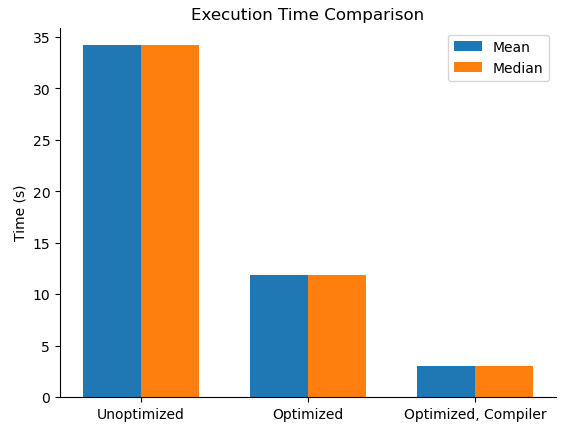
\includegraphics[height=.9\textheight]{../assets/ndim_first_bench.png}
\end{frame}

\begin{frame}{Cache-oblivious algorithms \cite{frigo}}
  \begin{columns}
    \begin{column}{0.5\textwidth}
      Standard Matrix Multiplication $A \cdot B$
      \begin{itemize}
        \item Traverses $A$ row-major order
        \item Traverses $B$ column-major order
          \begin{itemize}
            \item Every step of $B$ we get a cache miss
          \end{itemize}
        \item Solution: Transpose $B$
        \item $C_{ij}$ becomes row $A_i$ times \textbf{row} $B_j$
        \item Requires $\Theta(n^2)$ precompute.
          \begin{itemize}
            \item Does it improve speed?
            \item Does it reduce cache misses?
          \end{itemize}
      \end{itemize}
    \end{column}
    \begin{column}{0.5\textwidth}
      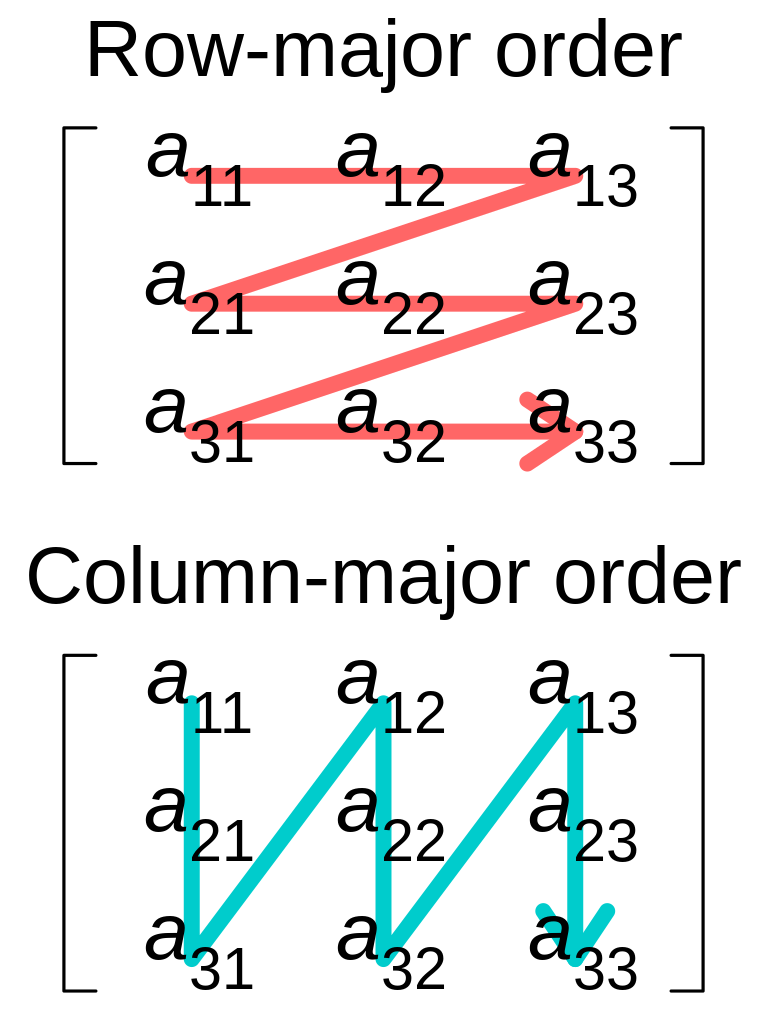
\includegraphics[height=0.9\textheight]{../assets/Row_and_column_major_order.svg.png}
      \cite{cmglee}
    \end{column}
  \end{columns}
\end{frame}

\begin{frame}{Cache-oblivious algorithms (cont.)}
  \begin{columns}
    \begin{column}{0.5\textwidth}
      \begin{block}{Does it improve Speed?}
        \begin{itemize}
          \item Lets benchmark it:
        \end{itemize}
  \begin{table}[h]
\begin{tabular}{|l|c|c|}
\hline
    & \textbf{Mean} & \textbf{Median}\\
\hline
    \textbf{Row-major} & $2.9668s$ & $2.9661 s$\\
  \hline
    \textbf{Col-major} & $2.1689 s$ & $2.1686 s$\\
\hline
\end{tabular}
\end{table}
      \end{block}
    \end{column}
    \pause
    \begin{column}{0.5\textwidth}
      \begin{block}{Does it reduce cache misses?}
        \begin{itemize}
          \item This is more complex
          \item For this, we have to simulate the caches
          \item This can be done using cachegrind \cite{valgrind}.
        \end{itemize}
      \end{block}
    \end{column}
  \end{columns}
\end{frame}

\begin{frame}{Iai \cite{iai}}
  \begin{columns}
    \begin{column}{0.5\textwidth}
  \begin{itemize}
    \item Based on cachegrind
    \item Emulating the CPU and its caches
    \item Precise single-shot measurements
    \item Main usecase in CI systems
  \end{itemize}
    \end{column}
    \pause
    \begin{column}{0.5\textwidth}
    \footnotesize\inputminted[xleftmargin=1em,linenos]{text}{../assets/iai.txt}
      \begin{itemize}
        \item Unclear, requires further investigation.
      \end{itemize}
    \end{column}
  \end{columns}
\end{frame}

\section{Parallelism}
\begin{frame}{SIMD}
  \begin{columns}
    \begin{column}{0.5\textwidth}
      \begin{block}{Old API}
        \begin{itemize}
          \item Experimental only; \textbf{Unsafe}
          \item Low level Platform-Specific structs
          \item Direct Intrincics translation
          \item Intel Documentation \cite{intel}:
            \begin{itemize}
              \item \texttt{\_\_mmask32 \_kadd\_mask32 (\_\_mmask32 a, \_\_mmask32 b)}
            \end{itemize}
          \item Rust port \cite{rustarch}:
            \begin{itemize}
              \item \texttt{unsafe fn \_kadd\_mask32(a: \_\_mmask32, b: \_\_mmask32) -> \_\_mmask32}
            \end{itemize}
        \end{itemize}
      \end{block}
    \end{column}
    \pause
    \begin{column}{0.5\textwidth}
      \begin{block}{Portable SIMD}
        \begin{itemize}
          \item Experimental only, \textbf{Safe}
          \item Generalized on \textbf{bit width level}
            \begin{itemize}
              \item \texttt{std::simd::\{f32x8, f64x4, i32x8\}}
            \end{itemize}
          \item Conditional Compilation \cite{concomp} with
            \begin{itemize}
              \item \texttt{\#[cfg(target\_arch="x86\_64")]}
              \item \texttt{\#[cfg(target\_feature="aes")]}
            \end{itemize}
          \item Conditional Execution \cite{isx86} with \texttt{std::is\_x86\_feature\_detected} (runtime)
        \end{itemize}
      \end{block}
    \end{column}
  \end{columns}
  \begin{center}
    Unable to port due to missing documentation
  \end{center}
\end{frame}

\begin{frame}{Rayon \cite{rayon}}
  \begin{itemize}
    \item High-Level Parallelism Library
    \item Gurantees \textbf{data-race freedom}
    \item Main Feature: Parallel Iterators
      \begin{itemize}
        \item Just replace \texttt{.iter()} with \texttt{.par\_iter()}
        \item Same functionality as sequential \textbf{if} the iterator has no side effects
        \item Support for High-Level functions
          \begin{itemize}
            \item \texttt{.map()}, \texttt{.filter()}, \texttt{.reduce()} \dots
          \end{itemize}
        \item Low level primitives such as \texttt{.join()}:
          \begin{itemize}
            \item \texttt{.join(|| a(), || b())}
            \item \textbf{May} run in parallel
            \item Based on if idle cores are available
          \end{itemize}
      \end{itemize}
  \end{itemize}
\end{frame}

\begin{frame}{Rayon (cond.)}
  \begin{tcolorbox}[title=Unported Code (no transpose)]
    \footnotesize\inputminted[xleftmargin=1em,linenos]{rust}{../assets/01rayon.rs}
  \end{tcolorbox}
\end{frame}

\begin{frame}{Rayon (cond.)}
  \begin{tcolorbox}[title=Ported to Iterators]
    \footnotesize\inputminted[xleftmargin=1em,linenos]{rust}{../assets/02rayon.rs}
  \end{tcolorbox}
\end{frame}

\begin{frame}{Rayon (cond.)}
  \begin{tcolorbox}[title=Ported to Iterators \textbf{and Parallelized!}]
    \footnotesize\inputminted[xleftmargin=1em,linenos]{rust}{../assets/03rayon.rs}
  \end{tcolorbox}
\end{frame}

\section{Conclusion}
\begin{frame}{Further Ressources}
  \begin{itemize}
    \item The Rust Performance Book \cite{perfbook}
      \begin{itemize}
        \item Bounds chacking
        \item I/O
        \item Perf linter clippy
        \item Type sizes
      \end{itemize}
      \pause
    \item Algorithmica: Algorithms for Modern Hardware \cite{algorithmica}
      \pause
    \item rsmpi \cite{mpi}
      \begin{itemize}
        \item Pure Rust implementation
        \item Compatible with
          \begin{itemize}
            \item OpenMPI
            \item MPICH
            \item MS-MPI (Windows)
          \end{itemize}
      \end{itemize}
  \end{itemize}
\end{frame}

\begin{frame}{Summary}
\label{pg:lastpage} % Label on last frame to get the page number for footer
  \begin{itemize}
    \item Rust is viable for HPC, although still experimental
      \pause
    \item There are many flags for compiler tuning
      \pause
    \item The following tools are available for HPC:
      \pause
  \end{itemize}
  \begin{table}[h]
\centering
    \begin{tabular}{|l|l|}
      \hline
      \textbf{Topic} & \textbf{Tool}\\
      \hline
      Microbenchmarking & Criterion\\
      \hline
      Application Benchmarking & Hyperfine\\
      \hline
      Assembly Generation & Compiler Explorer, cargo show-asm\\
      \hline
      Loop Unrolling & \texttt{unroll}, Compiler Arguments\\
      \hline
      Function Inlining & \texttt{\#[inline]} \\
      \hline
      Statistical Profiling & \texttt{cargo-flamegraph} \\
      \hline
      CI benchmarking & \texttt{iai} \\
      \hline
      SIMD & \texttt{std::simd}, \texttt{core::arch} \\
      \hline
      Intra-Node parallelism & rayon \\
      \hline
    \end{tabular}
  \end{table}
\end{frame}

\begin{frame}[allowframebreaks]{References}
\renewcommand*{\bibfont}{\normalfont\scriptsize}
\printbibliography
\end{frame}

\end{document}
